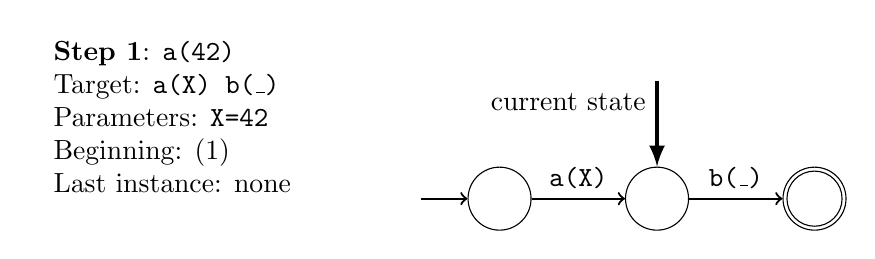
\begin{tikzpicture}[
    mystyle/.style={circle, minimum size=8mm, fill=white, draw=black}
]
    \node[mystyle] at (0,0) (n1) {};
    \node[mystyle] at (2,0) (n2) {};
    \node[mystyle] at (4,0) (n3) {};

    \draw[->, thick] (-1,0) -- (n1);
    \draw[->, thick] (n1) -- node[above] {\texttt{a(X)}} (n2);
    \draw[->, thick] (n2) -- node[above] {\texttt{b(\_)}} (n3);
    \draw[] (n3) circle (3.5mm);

    \draw[-latex, ultra thick] (2,1.5) -- node[near start, left] {current state} (n2);

    \node[anchor=west] at (-6,1) {\begin{tabular}{l}
        \textbf{Step 1}: \texttt{a(42)} \\
        Target: \texttt{a(X) b(\_)} \\
        Parameters: \texttt{X=42} \\
        Beginning: (1) \\
        Last instance: none
    \end{tabular}};
\end{tikzpicture}
